%%%%%%%%%%%%%%%%%%%%%%%%%%%%%%%%%%%%%%%%%%%%%%%%%%%%%%%%%%%%
%%% ELIFE ARTICLE TEMPLATE
%%%%%%%%%%%%%%%%%%%%%%%%%%%%%%%%%%%%%%%%%%%%%%%%%%%%%%%%%%%%
%%% PREAMBLE 
\documentclass[9pt,lineno,final]{elife}
% Use the onehalfspacing option for 1.5 line spacing
% Use the doublespacing option for 2.0 line spacing
% Please note that these options may affect formatting.
% Additionally, the use of the \newcommand function should be limited.


\usepackage{lipsum} % Required to insert dummy text
\usepackage[version=4]{mhchem}
\usepackage{siunitx}
\usepackage[color=green!30, textsize=small]{todonotes}
\usepackage{float}
\usepackage{graphicx}
\usepackage{grffile}
\usepackage{array}

\usepackage{algorithm2e}
\usepackage{cleveref} % use \cref or \Cref to refer to labeled elements for automatically referring to the right type of entity, with the right capital letter and/or abbreviation rules
\usepackage[subpreambles=true]{standalone}
% \usepackage{endfloat}
\DeclareSIUnit\Molar{M}

\newcommand{\pH}{\mathrm{pH}}
\newcommand{\pKa}{\mathrm{pKa}}

% Hidden table column
\newcolumntype{H}{>{\setbox0=\hbox\bgroup}c<{\egroup}@{}}
%%%%%%%%%%%%%%%%%%%%%%%%%%%%%%%%%%%%%%%%%%%%%%%%%%%%%%%%%%%%
%%% ARTICLE SETUP
%%%%%%%%%%%%%%%%%%%%%%%%%%%%%%%%%%%%%%%%%%%%%%%%%%%%%%%%%%%%
\title{Predicting pKa values and titration curves for the SAMPL6 pKa challenge using Epik and Jaguar}

\author[1,2]{Ari\"{e}n S. Rustenburg}
\author[1]{Mehtap Isik}
\author[1,2]{Patrick B. Grinaway}
\author[1,3]{Andrea Rizzi}
%\author[]{Art Bochevarov}
%\author[]{John Shelley}
\author[4]{Marilyn R Gunner}
\author[1*]{John D. Chodera}

\affil[1]{Computational and Systems Biology Program, Sloan Kettering Institute, Memorial Sloan Kettering Cancer Center, New York, NY 10065}
\affil[2]{Graduate Program in Physiology, Biophysics, and Systems Biology, Weill Cornell Medical College, New York, NY 10065}
\affil[3]{Tri-Institutional Training Program in Computational Biology and Medicine, New York, NY 10065}
\affil[4]{Department of Physics, City College of New York, New York, NY 10031}
\corr{john.chodera@choderalab.org}{JDC}

%\presentadd[\authfn{3}]{Schr\"{o}dinger, New York, NY 10036}

%\contrib[\authfn{1}]{These authors contributed equally to this work}
%\contrib[\authfn{2}]{These authors also contributed equally to this work}

%%%%%%%%%%%%%%%%%%%%%%%%%%%%%%%%%%%%%%%%%%%%%%%%%%%%%%%%%%%%
%%% ARTICLE START
%%%%%%%%%%%%%%%%%%%%%%%%%%%%%%%%%%%%%%%%%%%%%%%%%%%%%%%%%%%%

\begin{document}

\maketitle
%\tableofcontents
%\listoffigures
%\listoftables
\begin{abstract}
	The goal of the SAMPL6 pKa Challenge was to evaluate the performance of small molecule pKa prediction methods from challenge participants in a blinded fashion on a set of small, drug-like molecules resembling kinase inhibitor fragments.
	%
	To provide a useful point of comparison for blind participant predictions that may use experimental methods still under development, we performed reference benchmark calculations using a popular empirical model (Epik) and quantum chemical approach (Jaguar) from Schrödinger.
	%
	Epik predicts microstate populations and pKa values using a Hammett-Taft type model, while Jaguar is a fast DFT quantum chemical method.
	%
	In this work, we discuss how these reference calculations were performed, provide a broad assessment of the performance of the method, and highlight challenges and considerations in predicting pKa values to benchmark against experiment macroscopic pKa measurements.
\end{abstract}


\section{Introduction}

Titratable sites are ubiquitous in druglike small molecules.
%
Large-scale computational surveys suggest that 60\% of all protein-ligand complexes undergo a change in ionization state upon binding~\cite{Aguilar2010}, either due to protonation state changes of the small molecule or the protein (where roughly a third of all protein residues are ionizable~\cite{Jordan2005}).
%
More generally, protonation state effects---in which the dominant protonation, charge, or tautomer state shifts upon binding, or a mixture of protonation states are significantly populated in complex or solution---has the potential to cause large modeling errors if these effects are neglected. \cite{Martin2009, Greenwood2010,Bax2017}
%
In the SAMPL5 distribution coefficient (logD) challenge, for example, protonation state effects were determined to be a major contributor to loss in accuracy for the otherwise mundane task of predicting a transfer free energy between aqueous and cyclohexane phases~\cite{Pickard2016}.

To isolate the question of how well pKa effects could be modeled---and therefore how accurately the community could address these effects---the SAMPL6 challenge featured a blind pKa prediction component, as an intermediate step to logD predictions in which we provide participants with pKa values and later have them predict both pKa and logD~\cite{sampl6-pKa-measurements}.
The SAMPL6 pKa challenge consisted of predicting macroscopic pKa values measured by UV-metric titration for a set of small moelcules that resembled kinase inhibitors and their fragments~\cite{sampl6-pKa-measurements}.
As participants in the SAMPL6 pKa challenge were expected to utilize a wide variety of methods still under development, we endeavored to provide a useful baseline reference set of predictions using well-established, widely-deployed, commercially available methods.
We selected both an empirical method (Epik~\cite{Shelley2007Epik}) and quantum chemical method (Jaguar~\cite{Bochevarov2013}) from the Schr\"{o}dinger Suite of computational chemistry software, version 2017-4.

Reference calculations---which were not fully blinded---were performed in a manner that attempted to mimic standard use, using recommended settings for each program, without significantly modifying the input parameters.
As the computation of UV-metric macroscopic pKa values from the microscopic pKa values predicted by the tools is not necessarily completely straightforward, we considered several alternative possibilities, which we discuss in more detail.
We provide an analysis and broad assessment of the performance of the two methods, and highlight challenges and considerations in predicting pKa values to benchmark against experiment.
All analysis tools used to perform this study are available via GitHub at
\url{https://github.com/choderalab/SAMPL6-Reference-pKa-Calculations}

\section{Technology}


\subsection{Epik}

Epik\cite{Shelley2007Epik} is a program for predicting the pKa values of ionizable sites in druglike molecules and for generating their probable protonation states. Epik implements the empirical Hammett-Taft (HT) approach \cite{Perrin1981HammettTaft}  to rapidly estimate the pKa values of Brønsted acidic or basic functional groups identified by SMARTS \cite{SMARTSDaylight} patterns. The popular HT method describes a linear free energy relationship,

\begin{equation}
 pK_{a_i} = pK_{a_i}^0 - \rho_i  \sum_j \sigma_i \quad ,
\end{equation}

between an ionizable functional group reference $pK_{a_i}^0$ value, how sensitive (ρi) the group is to substituent perturbation, and how strongly ($\sigma_j$) each substituent, j, perturbs the pKa value. Epik’s internal $pK_{a_i}^0$, $\rho$ , and $\sigma$  parameters are fit to experimental data, or, rarely, to high-quality Jaguar calculations when experiments are unavailable.

Given a target pH and pH tolerance, the molecule can be appropriately protonated or deprotonated based on the estimated pKa values of its ionizable groups to generate the probable protonation states. The estimated pKa value of each functional group in a molecule is often exclusive to a specific tautomeric, protonation, and ionization state. Each (de)protonation can give rise to a set of tautomers and subsequent ionization states, all of which are iteratively generated and estimated until either exhausted or the predicted pKa values of the ionizable sites fall outside the tolerance range. Finally, the microscopic populations and corresponding free energy penalties are calculated and reported. Please note that Epik reports only microscopic pKa values, not macroscopic, or apparent pKa values.

\subsection{Jaguar}

Jaguar uses an \textit{ab initio} DFT method for calculating pKa values. 

It attempts to estimate the pKa using the free energy of deprotonation  

\begin{align}
 pK_a = \frac{\Delta G_\textrm{(aq)}}{RT \ln 10}  
\end{align}

The value of $ \Delta G_\textrm{(aq)}$ can be obtained using the following thermodynamic cycle:
%
\begin{figure}[H]
\centering
 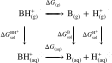
\includegraphics{jaguar-reaction}
\end{figure}
%
, which leads to the following equation.
%
\begin{equation}
 \Delta G_\textrm{(aq)} = \Delta G_\textrm{(g)} - \Delta G^\textrm{\ce{BH+}}_\textrm{sol} + \Delta G^\textrm{\ce{B}}_\textrm{sol}  +  \Delta G^\textrm{\ce{H+}}_\textrm{sol} \quad .
\end{equation}

From this equation, it follows that when the other 4 terms are known,
the pKa value can be estimated.

$\Delta G^\textrm{\ce{H+}}_\textrm{sol}$ has previously been established to be -259.5 kcal per mol\cite{Lim1991protonsolvation}.


Gas phase term $\Delta G_\textrm{(g)}$ is calculated using
%
\begin{equation}
 \Delta G_\textrm{(g)} = E_\textrm{\ce{B_{(g)}}} - E_\textrm{\ce{BH+ _{(g)}}} + \frac{5RT}{2 } - T \Delta S \quad .
\end{equation}


The energy terms require first a geometry optimization, which is performed using B3LYP/6-31G*. 
%
Afterwards, B3LYP/cc-pVTZ+ is used for atoms involved in the deprotonation reaction, and the remainder are treated using the cc-pVTZ basis set.
%
\todo[inline]{ASR: Describe solvation calculation and need for empirical correction}

\todo[inline]{ASR: Describe how multiple conformations are incorporated}
\todo[inline]{ASR:Explain the individual terms in the equations above, citations for method}

\section{Analysis}

\subsection{Microstate predictions}

Methods like Epik and Jaguar provide microstate pKa predictions.
%
This means that rather than macroscopic pKas observed in the average charge state (potentiometric titration) or number of titration events (UV titration curve), it produces a microequilibrium constant between a single pair of configurations (protonation states or tautomers) is predicted. 
%
One way to compare experiment and prediction is by directly comparing 
pKa values.
%
However, there are likely many microstates, and only a few macrostates.
%
Therefore, we also look at the predicted titration curve, which can incorporate information from every microstate into a macrostate.


\begin{figure}[H]
	\centering
	
	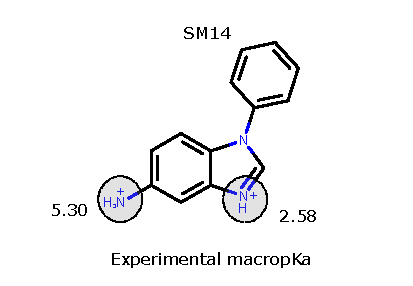
\includegraphics[width=0.47\textwidth]{Images/Molecules/SM14-pka.pdf} \hfill
	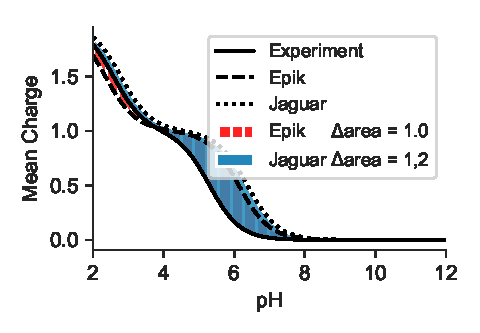
\includegraphics[width=0.47\textwidth]{fig1_charge_SM14.pdf} \\
    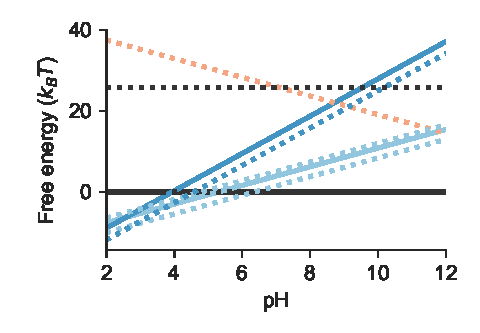
\includegraphics[width=0.47\textwidth]{fig1_free_energy_SM14.pdf} \hfill
	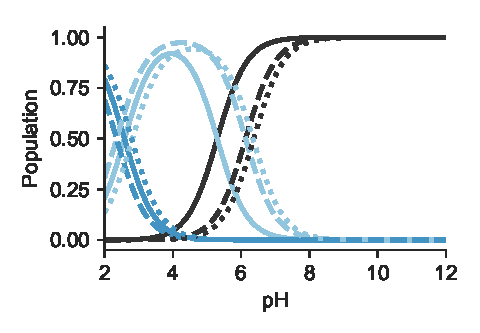
\includegraphics[width=0.47\textwidth]{fig1_population_SM14.pdf}\\
	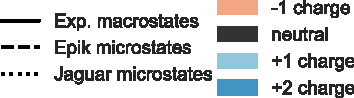
\includegraphics[width=0.4\textwidth]{fig1_legend.pdf}
	
		\caption{{\bf Epik and Jaguar microscopic pKa values can be used to generate free energies (bottom left) or, populations (bottom right), and recapitulate the binding curve (top right) when the charge of each species is added up.} Molecule SM14 pKa values (top left) were measured using UV (citation) for the purpose of the SAMPL6 challenge, and based on a subsequent NMR experiment the most likely sites of titration were established. We used Epik and Jaguar to predict microscopic pKa values (denoted as Type I predictions in SAMPL6). The macrostate populatons from experiment, and microstate populations from predictions can be compared directly to an experimental titration curve derived from UV. Since NMR data was available for this molecule, the charge state in the experiment is also known.
	\label{fig:sm14-prediction}}
	
\end{figure}





\subsection{Predicting macroscopic pKa values}

Epik and Jaguar predict microscopic pKa values or microstate energies, which must be translated into macroscopic pKa values for comparison to experiment.
Several choices are possible for comparing these microscopic properties into macroscopic pKa values.
%
It is also possible to translate the micropKas into macropKas
\cite{Philipp2018macropka}

\begin{align}
 K_a^\text{macro} = \sum_{j=1}^{N_\text{deprot}} \frac{1}{\sum_{i=1}^{N_\text{prot}}\frac{1}{ K_{ij^\text{micro}}}}
 \end{align}

\todo[inline]{See if I can perform those conversions for my data.}
 

\subsection{Population curves from pKa}

\begin{itemize}
	\item Description of the population curve generation from pKa \\
\end{itemize}

\begin{eqnarray}
	g_i(\pH) &=& \beta \left( n_i*\pH - \sum_j \pKa_j \right)
\end{eqnarray}

\begin{eqnarray}
	\pi_i(\pH) &=& \frac{e^{-g_i(\pH)}}{\sum_i e^{-g_i(\pH)} }
\end{eqnarray}

\subsection{Virtual electrochemical titration}


\begin{itemize}
	\item Description of the calculation of the mean charge curve \\
\end{itemize}

\begin{eqnarray}
	\langle q_\text{total} \rangle (\pH) = \sum_i q_i \times \pi_i(\pH) 
\end{eqnarray}



\begin{figure}[H]
	\centering
	
	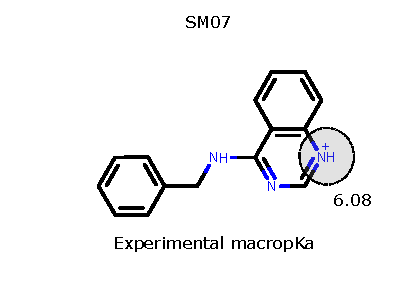
\includegraphics[width=0.47\textwidth]{Images/Molecules/SM07-pka.pdf} \hfill
	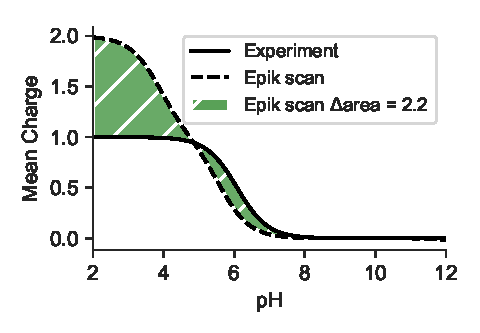
\includegraphics[width=0.47\textwidth]{fig2_charge_sm07.pdf} \\
	
    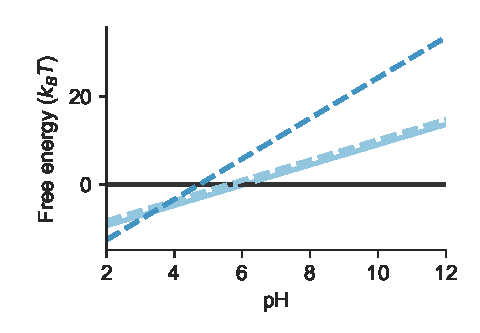
\includegraphics[width=0.47\textwidth]{fig2_free_energy_sm07.pdf}
    \hfill
	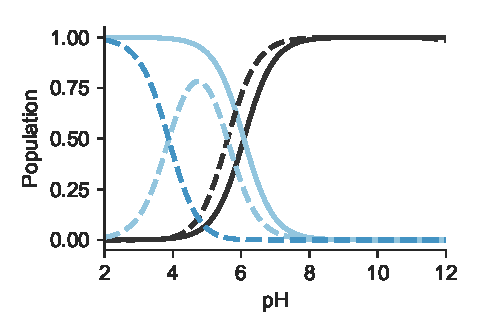
\includegraphics[width=0.47\textwidth]{fig2_population_sm07.pdf}\\
 	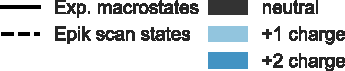
\includegraphics[width=0.4\textwidth]{fig2_legend}
	
		\caption{{\bf Epik scan provides sequential pKa values for adding single protons, which can approximate a macroscopic titration curve.} Molecule SM07 pKa values were measured using UV (citation) for the purpose of the SAMPL6 challenge, and based on a subsequent NMR experiment the identity of the microstates were identified. We used Epik scan mode to predict most prevalent microstates from sequential pKa values, which can approximate macroscopic pKa values. The macrostate populatons from experiment, and microstate populations from predictions can be compared directly to an experimental titration curve derived from UV pKa values. Since NMR data was available for this molecule, the charge identity in the experiment is also known. 
	\label{fig:scan-prediction}}
	
\end{figure}


\begin{itemize}
	\item Sequential titration avoids the need to compute the energies of \emph{all} protonation states
	\item Epik can automatically perform a sequential scan (which can also be used in Jaguar with some automation)
	\item For this experiment, we started from the predicted highest-occupancy microstate at pH 7 and went in both directions, returning pKa values between 2-12
	\item Average charge vs pH to match electrochemical titrations, look at the mean signed deviation (MSD) or area between curves to see whether the charge curve behavior matches
\end{itemize}


\section{Results}


\begin{table}[H]
\centering
	\caption{{\bf Overall performance of each method} using either the closest pKa matching, Hungarian pKa matching, or sequentially aligned pKa values, and the area between the experimental and predicted macroscopic charge titration curve}
	\label{tab:overview-performance}

\begin{tabular}{@{}cccccc@{}}
\toprule
              & \multicolumn{5}{c}{pKa}                                                  \\ \midrule
              & \multicolumn{5}{c}{RMSE}                                                 \\ \cmidrule(l){2-6} 
              & closest               &  & hungarian             &  & align              \\ \cmidrule(lr){2-2} \cmidrule(lr){4-4} \cmidrule(l){6-6} 
Epik micropka & 0.5; [0.3, 0.7]       &  & 0.5; [0.3, 0.7]       &  & \textemdash        \\
Epik scan     & 0.8; [0.6, 1.0]       &  & 0.8; [0.6, 1.0]       &  & 0.8; [0.6, 1.0]    \\
Jaguar        & 0.3; [0.2, 0.5]       &  & 0.3; [0.2, 0.5]       &  & \textemdash        \\
              &                       &  &                       &  &                    \\
              & \multicolumn{5}{c}{Pearson $\rho$}                                       \\ \cmidrule(l){2-6} 
              & closest               &  & hungarian             &  & align              \\ \cmidrule(lr){2-2} \cmidrule(lr){4-4} \cmidrule(l){6-6} 
Epik micropka & 0.96; [0.93, 0.99]    &  & 0.96; [0.92, 0.99]    &  & \textemdash        \\
Epik scan     & 0.94; [0.88, 0.97]    &  & 0.94; [0.87, 0.97]    &  & 0.94; [0.87, 0.97] \\
Jaguar        & 0.986; [0.966, 0.995] &  & 0.986; [0.969, 0.995] &  & \textemdash        \\ \midrule
              &                       &  &                       &  &                    \\
              & Charge vs pH          &  &                       &  &                    \\ \cmidrule(lr){2-2}
              & $\Delta$ area         &  &                       &  &                    \\ \cmidrule(lr){2-2}
Epik micropka & 1.8; [1.5, 2.1]       &  &                       &  &                    \\
Epik scan     & 1.7; [1.2, 2.2]       &  &                       &  &                    \\
Jaguar        & 1.5; [1.0, 2.1]       &  &                       &  &                    \\ \bottomrule
\end{tabular}
\end{table}


\begin{itemize}
	\item How much conformation-dependence is there in Jaguar-derived pKa values (or state energies)?
	\item Does sequential scan or mean molecular charge provide better agreement with experimental macroscopic pKa values? Would it be worthwhile to develop predictive UV-metric models?
	\item Comparison of observed accuracies to previously reported/expected accuracies; expected accuracy on kinase inhibitors derived from this study
	\item How does Epik compare to Jaguar in terms of accuracy and computational cost?
	\item Discussion of outliers
\end{itemize}




\subsection{Overall performance}

Some low probability structures produced by Epik included questionable protonation states of a heterycyclic moiety, present in SM03 and SM18 ( \Cref{fig:lewis-structure-SM03-SM18}). 



Overall performance of Epik and Jaguar based on various metrics (figures/tables)
\subsubsection {Matching of experimental and calculated pKa values}


The experiments do not provide any microscopic information on what atom, or microstate a pKa belongs to.
%
Therefore, it is necessary to perform a matching of pKa values between experiment and predicted pKa values.
%
There are several ways one could go about this, each strategy can prioritize a different aspect to match.
%
We consider three algorithms:
\paragraph{Closest pKa matching}
%

\begin{table}[H]
\centering
 \caption{{\bf Mean charge titration curve comparison with respect to experiment ($\Delta$ area) with confidence intervals.} Confidence intervals were obtained by gaussian bootstrapping over pKa values from the standard errors reported by the software.}\label{tab:titrationcurves}
 \begin{tabular}{lccc}
\toprule
 &    Epik micropka &           Jaguar &        Epik scan \\
Molecule &                  &                  &                  \\
\midrule
SM01     &  0.5; [0.2, 4.9] &  1.1; [0.0, 3.5] &  0.5; [0.1, 4.0] \\
SM02     &  2.1; [0.2, 3.1] &  1.6; [0.3, 5.3] &  1.9; [0.7, 4.2] \\
SM03     &  1.5; [1.0, 4.9] &  0.5; [0.8, 4.8] &  0.1; [0.2, 4.7] \\
SM04     &  2.6; [0.2, 4.0] &  1.1; [0.1, 4.0] &  2.2; [0.3, 5.0] \\
SM05     &  2.2; [0.6, 4.7] &  0.2; [0.1, 4.5] &  1.1; [0.5, 4.6] \\
SM06     &  2.2; [0.7, 9.5] &  1.3; [0.6, 4.7] &  2.6; [0.6, 6.8] \\
SM07     &  2.6; [0.1, 4.1] &  0.8; [0.1, 4.1] &  2.2; [0.7, 4.8] \\
SM08     &  1.2; [0.5, 6.2] &  7.1; [3.3, 9.2] &  0.6; [0.1, 5.8] \\
SM09     &  2.5; [0.3, 3.4] &  1.0; [0.1, 4.3] &  2.3; [0.6, 3.3] \\
SM10     &  0.6; [0.2, 5.1] &  0.3; [0.2, 5.3] &  0.6; [0.1, 5.6] \\
SM11     &  1.9; [0.2, 4.1] &  3.9; [0.5, 6.8] &  0.1; [0.2, 5.0] \\
SM12     &  2.5; [0.2, 3.4] &  0.9; [0.4, 4.7] &  2.2; [1.1, 3.6] \\
SM13     &  2.6; [0.2, 3.8] &  0.5; [0.1, 4.0] &  2.8; [0.3, 5.0] \\
SM14     &  1.0; [0.8, 5.4] &  1.2; [0.1, 4.1] &  1.8; [0.6, 5.2] \\
SM15     &  1.1; [0.4, 4.6] &  0.3; [0.2, 2.4] &  1.3; [0.4, 4.2] \\
SM16     &  2.9; [0.7, 4.7] &  1.5; [0.5, 4.4] &  1.4; [0.6, 4.7] \\
SM17     &  1.7; [0.1, 3.2] &  0.1; [0.0, 1.6] &  1.7; [0.2, 3.1] \\
SM18     &  0.8; [1.2, 9.7] &  2.2; [1.5, 7.9] &  1.0; [1.1, 8.2] \\
SM19     &  0.7; [0.2, 5.2] &  1.8; [0.6, 6.7] &  0.7; [0.2, 5.9] \\
SM20     &  2.3; [0.1, 4.7] &  1.6; [0.2, 3.4] &  2.3; [0.1, 4.8] \\
SM21     &  2.2; [0.8, 5.5] &  1.6; [0.5, 7.0] &  0.5; [0.4, 6.7] \\
SM22     &  1.6; [0.5, 4.8] &  0.2; [0.1, 3.4] &  1.6; [0.3, 3.9] \\
SM23     &  0.4; [0.2, 3.5] &  2.1; [0.7, 5.7] &  3.1; [1.9, 4.8] \\
SM24     &  3.6; [0.1, 5.0] &  2.3; [0.2, 4.9] &  5.6; [3.0, 8.6] \\
\bottomrule
\end{tabular}
 
\end{table}



\begin{figure}[hbtp]
\centering
\todo[inline,color=red!20]{ASR: Update these with latest version with correct rho/rmse values}
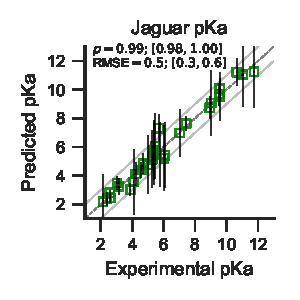
\includegraphics[scale=1.2]{closest_pka_jaguar.pdf}
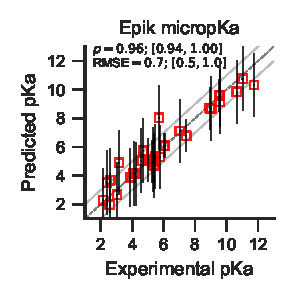
\includegraphics[scale=1.2]{closest_pka_epik_micropka.pdf}
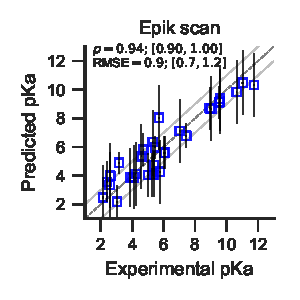
\includegraphics[scale=1.2]{closest_pka_epik_scan.pdf}
\caption{{\bf Comparison of computed pKa values to experimental macroscopic pKa values.} {\it Left:} Microscopic pKa values for Jaguar were matched ot the experimental dataset using \cref{alg:closest}. An alternative alignment of pKa values using the Hungarian algorithm (\cref{alg:hungarian}) is available as a supplementary figure.
{\it Middle:} Microscopic pKa values for Epik were matched ot the experimental dataset using \cref{alg:closest}. An alternative alignment of pKa values using the Hungarian algorithm (\cref{alg:hungarian}) is available as a supplementary figure.
{\it Right:} Macroscopic pKa values for Jaguar were matched ot the experimental dataset using \cref{alg:closest}. An alternative alignment of pKa values using the Hungarian algorithm (\cref{alg:hungarian}) is available as a supplementary figure. \label{correlation-closest}}


\end{figure}

%
\paragraph{Hungarian pKa matching}
This algorithm, also known as linear sum assignment.
%
It finds the combination of pKa that minimizes the overall cost by picking rows and columns in a matrix, also considering the cost of not mapping certain pKa values in the case of different numbers of predictions and experimental values.
%
The results do not seem to differ from closest-pka matching.

\paragraph{Sequential pKa matching}

For macroscopic only, because it doesn't make sense to sequentially align microscopic pKa values to a set of macroscopic pKa values
\cref{alg:sequential}

\begin{figure}[hbtp]
	\centering
	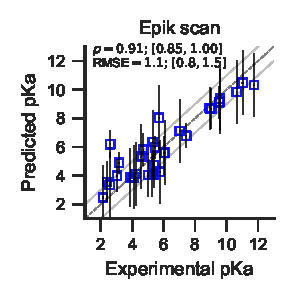
\includegraphics[scale=1.2]{aligned_pka_epik_scan.pdf}	
	\caption{{\bf Epik macroscopic pKa values compared to macroscopic experimental pKa values, sequentially matching pKa values}
		Comparison of the Epik sequential scan with entire experimental data set is shown, allowing only sequential pKa values to match experiment.\label{fig:correlation-sequential}}
\end{figure}
    

 
 \sisetup{separate-uncertainty=true}
\begin{table}
\centering
\caption{{\bf Macroscopic pKa values computed via Epik's sequential scan procedure.}
		Experimental and computed pKa values matched using sequential alignment of pKa values.}
\label{tab:molecule-macro}
\rowcolors{2}{gray!25}{white}
\begin{tabular}{cS[table-format=-1.2,table-figures-uncertainty=1]S[table-format=-1.1,table-figures-uncertainty=1]S[table-format=-1.1,table-figures-uncertainty=1]}\toprule
{Molecule} &  {Experimental} &  {Epik-scan} \\
\midrule
      SM01 &   9.53 \pm 0.01 &      9 \pm 1 \\
      SM02 &   5.03 \pm 0.01 &      4 \pm 1 \\
      SM03 &   7.02 \pm 0.01 &      7 \pm 2 \\
      SM04 &   6.02 \pm 0.01 &      6 \pm 1 \\
      SM05 &   4.59 \pm 0.01 &      5 \pm 2 \\
      SM06 &   3.03 \pm 0.04 &      4 \pm 1 \\
      SM06 &  11.74 \pm 0.01 &     10 \pm 2 \\
      SM07 &   6.08 \pm 0.01 &      6 \pm 2 \\
      SM08 &   4.22 \pm 0.01 &      4 \pm 2 \\
      SM09 &   5.37 \pm 0.01 &  4.0 \pm 0.9 \\
      SM10 &   9.02 \pm 0.01 &      9 \pm 1 \\
      SM11 &   3.89 \pm 0.01 &      4 \pm 2 \\
      SM12 &   5.28 \pm 0.01 &      4 \pm 1 \\
      SM13 &   5.77 \pm 0.01 &      4 \pm 2 \\
      SM14 &   2.58 \pm 0.01 &      3 \pm 2 \\
      SM14 &   5.30 \pm 0.01 &      6 \pm 2 \\
      SM15 &   4.70 \pm 0.01 &      6 \pm 1 \\
      SM15 &   8.94 \pm 0.01 &      9 \pm 1 \\
      SM16 &   5.37 \pm 0.01 &  4.7 \pm 0.9 \\
      SM16 &  10.65 \pm 0.01 &     10 \pm 2 \\
      SM17 &   3.16 \pm 0.01 &  4.9 \pm 0.7 \\
      SM18 &   2.15 \pm 0.02 &      2 \pm 2 \\
      SM18 &   9.58 \pm 0.03 &      9 \pm 2 \\
      SM18 &  11.02 \pm 0.04 &     10 \pm 2 \\
      SM19 &   9.56 \pm 0.02 &      9 \pm 2 \\
      SM20 &   5.70 \pm 0.03 &      8 \pm 2 \\
      SM21 &   4.10 \pm 0.01 &      4 \pm 2 \\
      SM22 &   2.40 \pm 0.02 &      4 \pm 1 \\
      SM22 &   7.43 \pm 0.01 &  6.8 \pm 0.9 \\
      SM23 &   5.45 \pm 0.01 &  6.0 \pm 0.8 \\
      SM24 &   2.60 \pm 0.01 &      4 \pm 1 \\
\bottomrule
\end{tabular}
\end{table}


\subsection{Macroscopic titration curves}
\begin{itemize}
	\item Compare macroscopic titration results
	\item different types of mistakes
	\begin{enumerate}
	 \item wrong pKa value 
	 \item too many pKa values (wrong total charges)
	\end{enumerate}

\end{itemize}




\sisetup{separate-uncertainty=true}
\begin{table}[H]
\centering
\caption{{\bf Microscopic pKa per molecule for each method as matched by the "closest" algorithm (\cref{alg:closest}), compared to experiment.} The uncertainty indicated is the standard error from the experiment, and the reported standard error by the prediction method.}
	\label{tab:molecule-micro-closest}
\rowcolors{2}{gray!25}{white}
\todo[inline]{Add deviation from experiment columns}
\begin{tabular}{cS[table-format=-1.2,table-figures-uncertainty=1]S[table-format=-1.1,table-figures-uncertainty=1]S[table-format=-1.1,table-figures-uncertainty=1]S[table-format=-1.1,table-figures-uncertainty=1]S[table-format=-1.1,table-figures-uncertainty=1]}\toprule
{Molecule} &  {Experimental} & {Epik-micropka} &      {Jaguar} &  {Epik-scan} \\
\midrule
      SM01 &   9.53 \pm 0.01 &        10 \pm 1 &   9.7 \pm 0.8 &      9 \pm 1 \\
      SM02 &   5.03 \pm 0.01 &         5 \pm 1 &       5 \pm 2 &      4 \pm 1 \\
      SM03 &   7.02 \pm 0.01 &         7 \pm 2 &       7 \pm 2 &      7 \pm 2 \\
      SM04 &   6.02 \pm 0.01 &     6.1 \pm 0.9 &       5 \pm 2 &      6 \pm 1 \\
      SM05 &   4.59 \pm 0.01 &         5 \pm 2 &   4.4 \pm 0.5 &      5 \pm 2 \\
      SM06 &   3.03 \pm 0.04 &         3 \pm 2 &   3.5 \pm 0.5 &  2.2 \pm 0.9 \\
      SM06 &  11.74 \pm 0.01 &        10 \pm 2 &      11 \pm 2 &     10 \pm 2 \\
      SM07 &   6.08 \pm 0.01 &     6.1 \pm 0.9 &       5 \pm 2 &      6 \pm 2 \\
      SM08 &   4.22 \pm 0.01 &         4 \pm 2 &   4.1 \pm 0.8 &      4 \pm 2 \\
      SM09 &   5.37 \pm 0.01 &         5 \pm 1 &       6 \pm 2 &  4.0 \pm 0.9 \\
      SM10 &   9.02 \pm 0.01 &         9 \pm 2 &       9 \pm 2 &      9 \pm 1 \\
      SM11 &   3.89 \pm 0.01 &         4 \pm 2 &   3.0 \pm 0.4 &      4 \pm 2 \\
      SM12 &   5.28 \pm 0.01 &         5 \pm 1 &       5 \pm 2 &      4 \pm 1 \\
      SM13 &   5.77 \pm 0.01 &         5 \pm 2 &       5 \pm 2 &      4 \pm 2 \\
      SM14 &   5.30 \pm 0.01 &         5 \pm 2 &   5.3 \pm 0.7 &      6 \pm 2 \\
      SM14 &   2.58 \pm 0.01 &         3 \pm 2 &   2.8 \pm 0.1 &      3 \pm 2 \\
      SM15 &   8.94 \pm 0.01 &         9 \pm 1 &   8.7 \pm 0.8 &      9 \pm 1 \\
      SM15 &   4.70 \pm 0.01 &         6 \pm 1 &   4.8 \pm 0.7 &      6 \pm 1 \\
      SM16 &   5.37 \pm 0.01 &         5 \pm 2 &       6 \pm 2 &  4.7 \pm 0.9 \\
      SM16 &  10.65 \pm 0.01 &        10 \pm 2 &  11.2 \pm 0.9 &     10 \pm 2 \\
      SM17 &   3.16 \pm 0.01 &     4.9 \pm 0.8 &   3.2 \pm 0.6 &  4.9 \pm 0.7 \\
      SM18 &   9.58 \pm 0.03 &        10 \pm 2 &      10 \pm 2 &      9 \pm 2 \\
      SM18 &   2.15 \pm 0.02 &         2 \pm 2 &       2 \pm 2 &      2 \pm 2 \\
      SM18 &  11.02 \pm 0.04 &        11 \pm 2 &      11 \pm 2 &     10 \pm 2 \\
      SM19 &   9.56 \pm 0.02 &         9 \pm 2 &  10.1 \pm 0.7 &      9 \pm 2 \\
      SM20 &   5.70 \pm 0.03 &         8 \pm 2 &   7.3 \pm 0.9 &      8 \pm 2 \\
      SM21 &   4.10 \pm 0.01 &         4 \pm 2 &       4 \pm 2 &      4 \pm 2 \\
      SM22 &   7.43 \pm 0.01 &     6.8 \pm 0.9 &   7.6 \pm 0.5 &  6.8 \pm 0.9 \\
      SM22 &   2.40 \pm 0.02 &         4 \pm 2 &   2.4 \pm 0.5 &      4 \pm 1 \\
      SM23 &   5.45 \pm 0.01 &         5 \pm 2 &       6 \pm 2 &  6.0 \pm 0.8 \\
      SM24 &   2.60 \pm 0.01 &         4 \pm 2 &   2.5 \pm 0.3 &      4 \pm 1 \\
\bottomrule
\end{tabular}
\end{table}




    
\begin{figure}[hbtp]
	\centering	
	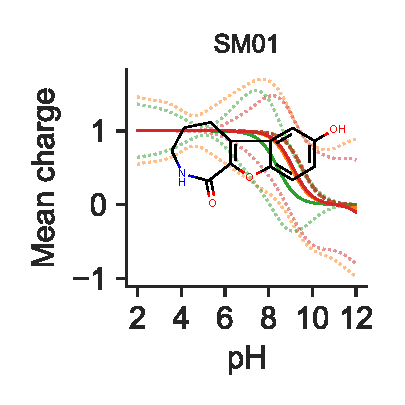
\includegraphics[width=0.33\textwidth]{Reports/SM01-titrationcurve-views.pdf}
	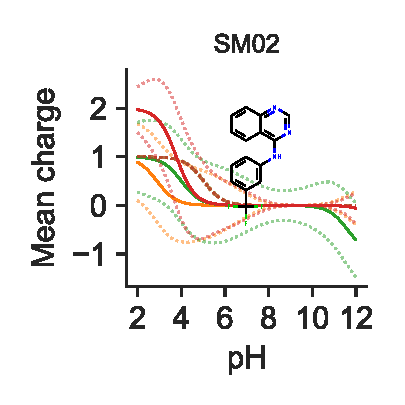
\includegraphics[width=0.33\textwidth]{Reports/SM02-titrationcurve-views.pdf}
	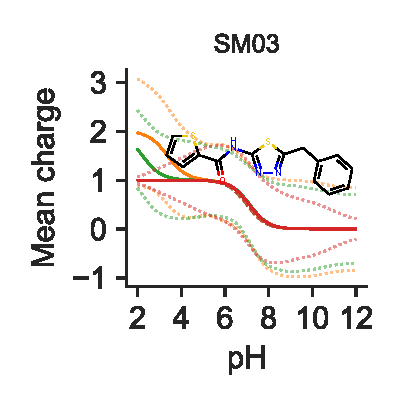
\includegraphics[width=0.33\textwidth]{Reports/SM03-titrationcurve-views.pdf}	 \\
    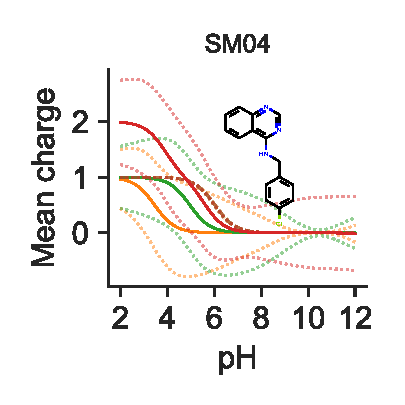
\includegraphics[width=0.33\textwidth]{Reports/SM04-titrationcurve-views.pdf}
	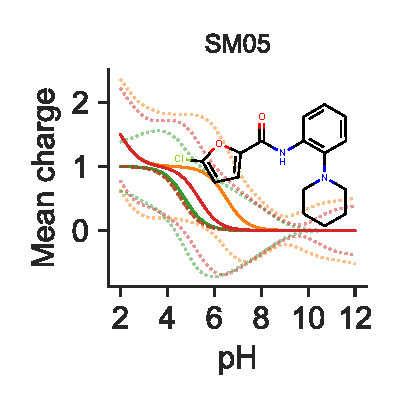
\includegraphics[width=0.33\textwidth]{Reports/SM05-titrationcurve-views.pdf}
	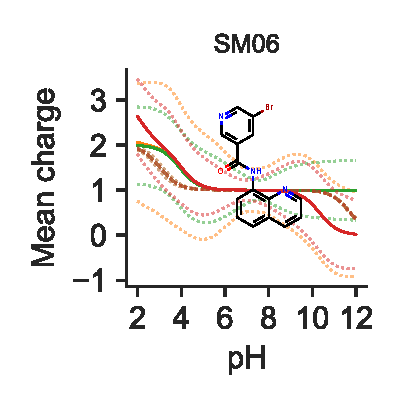
\includegraphics[width=0.33\textwidth]{Reports/SM06-titrationcurve-views.pdf}	 \\
		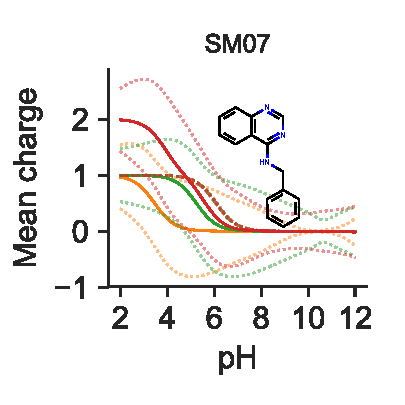
\includegraphics[width=0.33\textwidth]{Reports/SM07-titrationcurve-views.pdf}
	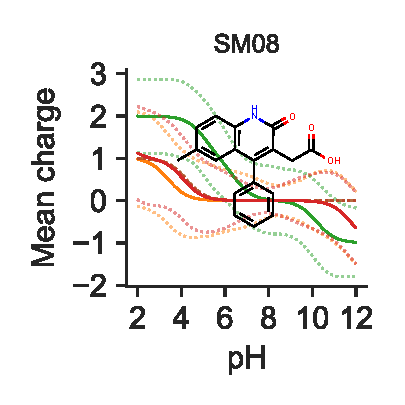
\includegraphics[width=0.33\textwidth]{Reports/SM08-titrationcurve-views.pdf}
	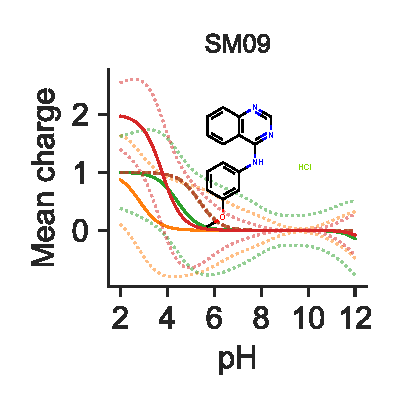
\includegraphics[width=0.33\textwidth]{Reports/SM09-titrationcurve-views.pdf}	 \\
	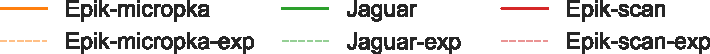
\includegraphics[]{Reports/overview-legend.pdf}
	\caption{{\bf Bootstrap titration curves for each method compared to experiment for molecules SM01-SM09.} The titration curve for each method is shown as a solid line, and 96 \% confidence intervals from bootstrap have been shown as dotted lines. Since the absolute experimental charge is not available in general, experimental curves (dashed) were aligned to each prediction independently using an integer offset that minimizes the area between curves. A numerical comparison to experiment is presented in \cref{tab:titrationcurves}.
	\label{fig:charge-curves1}}
	\end{figure}
	
	
\begin{figure}[hbtp]	
	\centering
	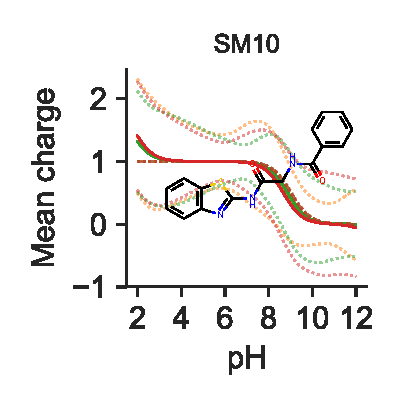
\includegraphics[width=0.33\textwidth]{Reports/SM10-titrationcurve-views.pdf}
	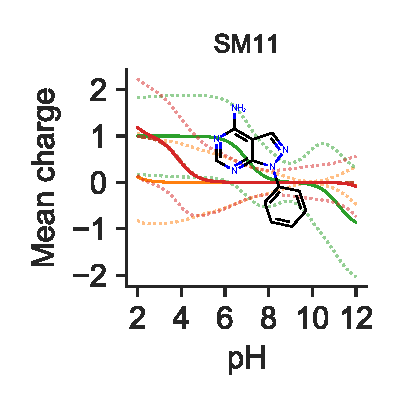
\includegraphics[width=0.33\textwidth]{Reports/SM11-titrationcurve-views.pdf}
	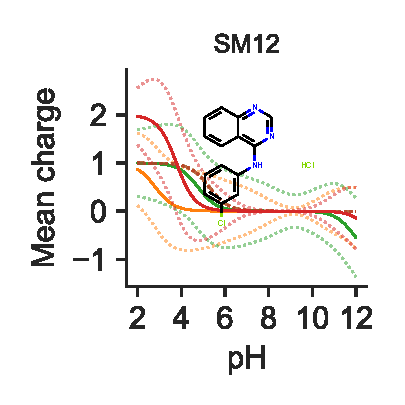
\includegraphics[width=0.33\textwidth]{Reports/SM12-titrationcurve-views.pdf}	 \\
	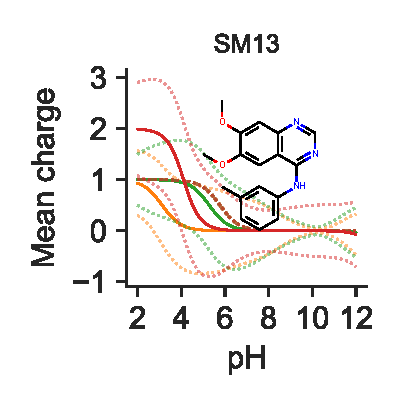
\includegraphics[width=0.33\textwidth]{Reports/SM13-titrationcurve-views.pdf}
	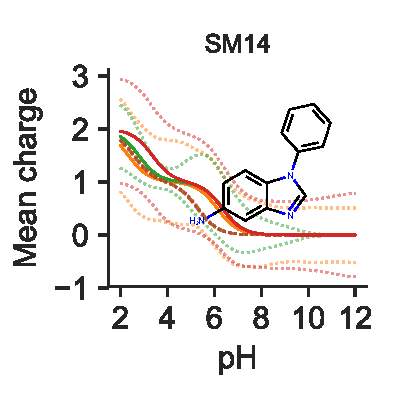
\includegraphics[width=0.33\textwidth]{Reports/SM14-titrationcurve-views.pdf}
	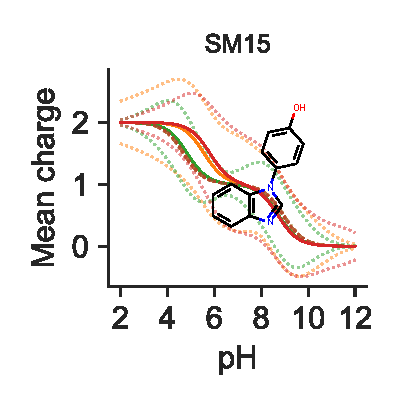
\includegraphics[width=0.33\textwidth]{Reports/SM15-titrationcurve-views.pdf}	 \\
	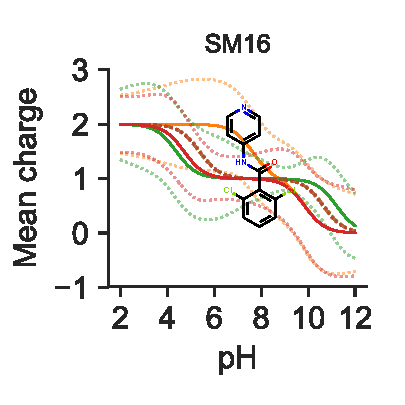
\includegraphics[width=0.33\textwidth]{Reports/SM16-titrationcurve-views.pdf}
	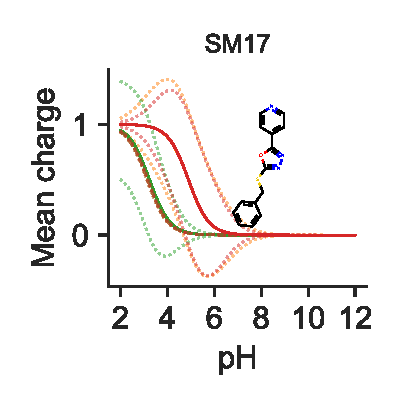
\includegraphics[width=0.33\textwidth]{Reports/SM17-titrationcurve-views.pdf}
	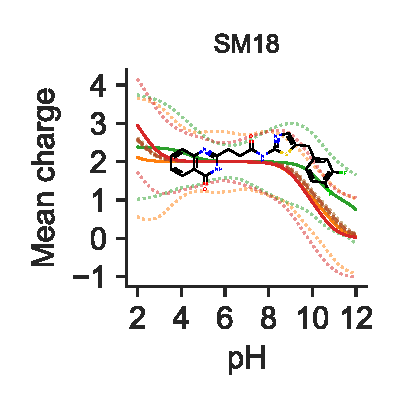
\includegraphics[width=0.33\textwidth]{Reports/SM18-titrationcurve-views.pdf}	 \\
	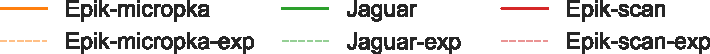
\includegraphics[]{Reports/overview-legend.pdf}

	\caption{{\bf Bootstrap titration curves for each method compared to experiment for molecules SM10-SM18.} The titration curve for each method is shown as a solid line, and 96 \% confidence intervals from bootstrap have been shown as dotted lines. Since the absolute experimental charge is not available in general, experimental curves (dashed) were aligned to each prediction independently using an integer offset that minimizes the area between curves. A numerical comparison to experiment is presented in \cref{tab:titrationcurves}.
	\label{fig:charge-curves2}}

\end{figure}
    
 \begin{figure}[hbtp]	
	\centering
	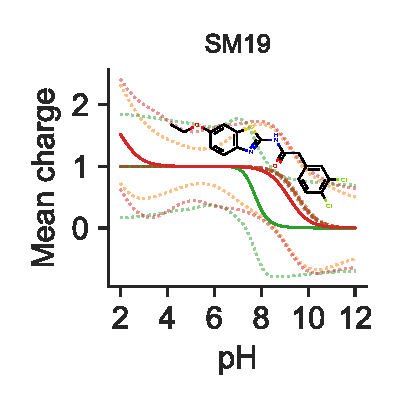
\includegraphics[width=0.33\textwidth]{Reports/SM19-titrationcurve-views.pdf}
	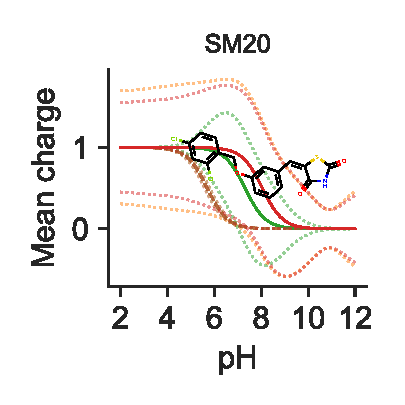
\includegraphics[width=0.33\textwidth]{Reports/SM20-titrationcurve-views.pdf}
	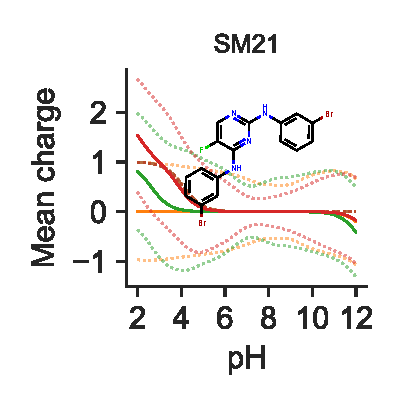
\includegraphics[width=0.33\textwidth]{Reports/SM21-titrationcurve-views.pdf}	 \\
	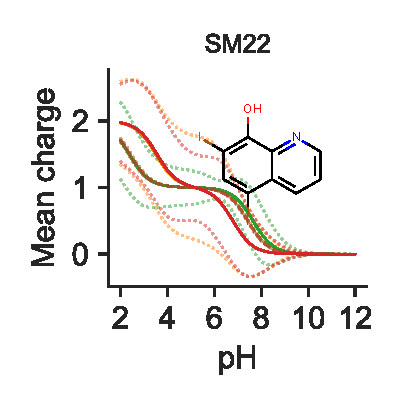
\includegraphics[width=0.33\textwidth]{Reports/SM22-titrationcurve-views.pdf}
	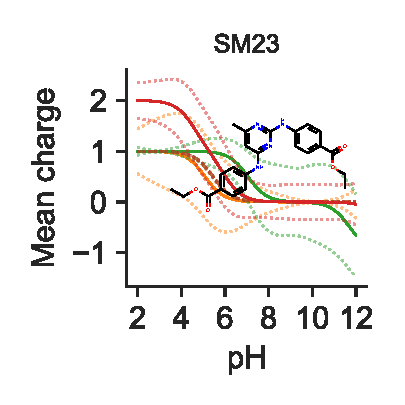
\includegraphics[width=0.33\textwidth]{Reports/SM23-titrationcurve-views.pdf}
	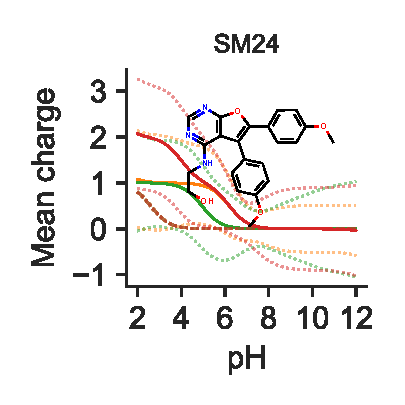
\includegraphics[width=0.33\textwidth]{Reports/SM24-titrationcurve-views.pdf}	 \\
    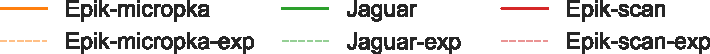
\includegraphics[]{Reports/overview-legend.pdf}

	\caption{{\bf Bootstrap titration curves for each method compared to experiment for molecules SM19-SM24.} The titration curve for each method is shown as a solid line, and 96 \% confidence intervals from bootstrap have been shown as dotted lines. Since the absolute experimental charge is not available in general, experimental curves (dashed) were aligned to each prediction independently using an integer offset that minimizes the area between curves. A numerical comparison to experiment is presented in \cref{tab:titrationcurves}.
	\label{fig:charge-curves3}}
	

\end{figure}

\section{Discussion}


\subsection{Problematic Lewis structures}
Epik generates some structures that seem to have invalid lewis structures.
\cref{fig:lewis-structure-SM03-SM18}.

\begin{figure}[H]	
\centering
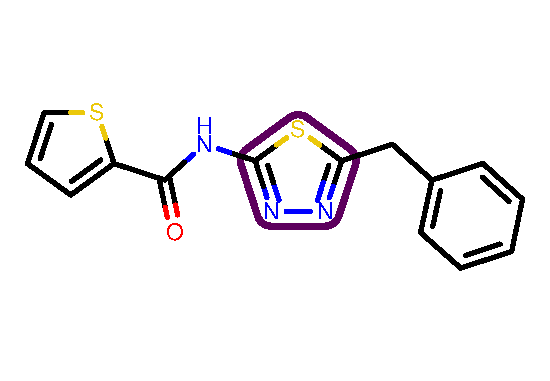
\includegraphics[width=0.33\textwidth]{Images/Molecules/SM03-smarts.pdf}
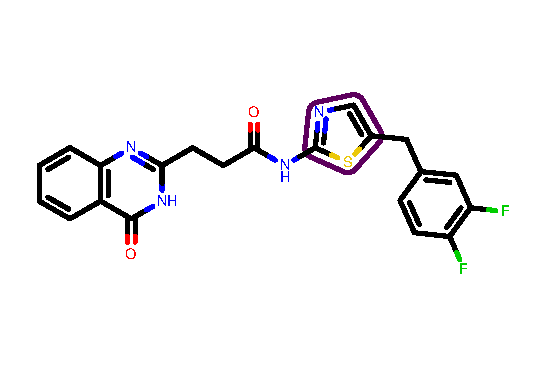
\includegraphics[width=0.33\textwidth]{Images/Molecules/SM18-smarts.pdf}
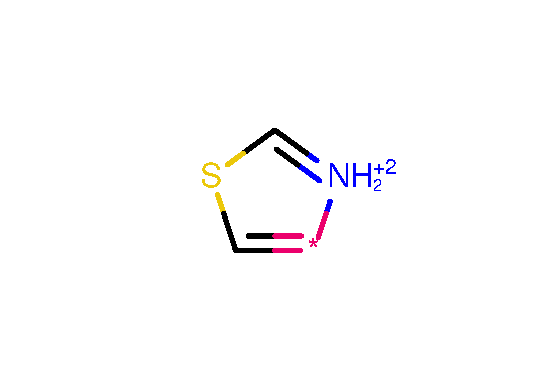
\includegraphics[width=0.33\textwidth]{Images/Molecules/lewis-problem.pdf}
\caption{{\bf Problematic lewis structure generated by Epik.}
Epik generated protonation states with invalid Lewis structure for SM03 and SM18, with a pentavalent nitrogen present in the thiazole/thiadiazole (the protonation pattern displayed on the right). One of these was also present in the set provided as part of SAMPL6  microstates, namely SM03\textunderscore{}micro021. A valid Lewis structure could not be figured out for this protonation state.}
\label{fig:lewis-structure-SM03-SM18}
\end{figure}		

\subsection{Descriptor analysis}
\begin{itemize}
	\item which moieties are harder to predict?
	\item Do certain descriptors correlate with variance/absolute errors?
	\item Do number of rotatable bonds affect epik/jaguar results (conformations missing from prediction)?
\end{itemize}


\subsection{Suggestions for future challenges}
\begin{itemize}
	\item Future challenges could benefit from NMR experiments for microstates
	\item Potentiometric titrations could capture states that may have been left out
	\item Probabilistic models (i.e. bayesian hierarchical models) could be constructed for the analysis of experiments. 
\end{itemize}

\section{Conclusions}

\begin{itemize}
	\item Epik and Jaguar perform well when matching both pKa and curves
	\item Microscopic pKa comparison directly to macroscopic may be deceiving, so the titration curve pose an alternative interpretation that can help assess
	\item Epik has a few artifacts (weird states, state penalties)
	\item future challenges could benefit from more NMR experiments and potentiometric titration data
	\item How a future challenge could make this easier
\end{itemize}


\section{Methods}


\subsection{Epik micropKa predictions}
\begin{itemize}
	\item were performed between pH 2-12
	\item Reported states with a minimum population of $e^{-10/RT}$
	\item States proposed by SAMPL6 but not predicted by Epik were not considered in analysis.
	      
\end{itemize}

\subsection{Epik scan: Sequential titration of dominant species} 


Started at pH 7.0, add protons sequentially. 
%
Produces the dominant microspecies as a way to mimic the likely macrostate.
%


\subsection{Jaguar: Ab initio quantum chemical pKa predictions}
\begin{itemize}
	\item Ran using default settings (5 conformations) for each of the pre-enumerated specified microstate pairs.
	\item Input structures were first minimized using MMFF.
	\item Additional minimization was performed for structures for which scf/geopt did not converge
\end{itemize}




%%%%%%%%%%%%%%%%%%%%%%%%%%%%%%%%%%%%%%%%%%%%%%%%%%%%%%%%%%%%%%%%%%%%%%%%%%%%%%%%%%%%%%%%%%%%%%%%%%%%%
% Code and Data Availability
%%%%%%%%%%%%%%%%%%%%%%%%%%%%%%%%%%%%%%%%%%%%%%%%%%%%%%%%%%%%%%%%%%%%%%%%%%%%%%%%%%%%%%%%%%%%%%%%%%%%%%

\section{Code and data availability}

\begin{itemize}
	\item Input files and analysis scripts are available at \href{https://github.com/choderalab/SAMPL6-reference-pka-calculations}{https://github.com/choderalab/SAMPL6-reference-pka-calculations}
\end{itemize}

%%%%%%%%%%%%%%%%%%%%%%%%%%%%%%%%%%%%%%%%%%%%%%%%%%%%%%%%%%%%%%%%%%%%%%%%%%%%%%%%%%%%%%%%%%%%%%%%%%%%%%
% Author Contributions 
%%%%%%%%%%%%%%%%%%%%%%%%%%%%%%%%%%%%%%%%%%%%%%%%%%%%%%%%%%%%%%%%%%%%%%%%%%%%%%%%%%%%%%%%%%%%%%%%%%%%%%
\section{Author Contributions}

\todo[inline]{(Follow the \href{http://www.cell.com/pb/assets/raw/shared/guidelines/CRediT-taxonomy.pdf}{CRediT Taxonomy})}

%%%%%%%%%%%%%%%%%%%%%%%%%%%%%%%%%%%%%%%%%%%%%%%%%%%%%%%%%%%%%%%%%%%%%%%%%%%%%%%%%%%%%%%%%%%%%%%%%%%%%%
% Acknowledgments 
%%%%%%%%%%%%%%%%%%%%%%%%%%%%%%%%%%%%%%%%%%%%%%%%%%%%%%%%%%%%%%%%%%%%%%%%%%%%%%%%%%%%%%%%%%%%%%%%%%%%%%
\section{Acknowledgments}

ASR, MI, AR, PBG, and JDC acknowledge support from the Sloan Kettering Institute.
JDC acknowledges support from NIH grant P30 CA008748.

%%%%%%%%%%%%%%%%%%%%%%%%%%%%%%%%%%%%%%%%%%%%%%%%%%%%%%%%%%%%%%%%%%%%%%%%%%%%%%%%%%%%%%%%%%%%%%%%%%%%%%
% Disclosures 
%%%%%%%%%%%%%%%%%%%%%%%%%%%%%%%%%%%%%%%%%%%%%%%%%%%%%%%%%%%%%%%%%%%%%%%%%%%%%%%%%%%%%%%%%%%%%%%%%%%%%%
\section{Disclosures}

JDC is a member of the Scientific Advisory Board for Schr\"{o}dinger, LLC.

\bibliography{sampl6-pKa-prediction}

%%%%%%%%%%%%%%%%%%%%%%%%%%%%%%%%%%%%%%%%%%%%%%%%%%%%%%%%%%%%
%%% APPENDICES
%%%%%%%%%%%%%%%%%%%%%%%%%%%%%%%%%%%%%%%%%%%%%%%%%%%%%%%%%%%%


\appendix

\section{Supplementary Information}



% \documentclass[11pt,final]{article}
\renewcommand{\familydefault}{\sfdefault}
\usepackage[utf8]{inputenc}
\usepackage[english]{babel}
\usepackage[showframe]{geometry}
\geometry{letterpaper}
\geometry{margin=1in}
\usepackage{graphicx}

\begin{document}
\newcommand{\molid}{SM01}
\newcommand{\methoda}{Epik-TypeI}
\newcommand{\methodb}{Jaguar-TypeI}
\newcommand{\methodc}{Epik-TypeII}
\newcommand{\methodd}{Epik-TypeIII}

\noindent 
\begin{minipage}[s]{0.35\textwidth}\centering
\includegraphics[width=\textwidth]{\molid-molecule.png}
\end{minipage}
\begin{minipage}[s]{0.35\textwidth}
\includegraphics[width=\textwidth]{overview-virtual-titration-\molid.png}
\end{minipage}
\begin{minipage}[s]{0.23\textwidth}
\includegraphics[width=\textwidth]{overview-legend-\molid.png}
\end{minipage}

\begin{minipage}[s]{\textwidth}\centering
{\textbf \methoda}
\end{minipage}

\noindent
\begin{minipage}[s]{0.32\textwidth}\centering
\includegraphics[width=\textwidth]{\methoda-virtual-titration-\molid.png}
\end{minipage}
\begin{minipage}[s]{0.32\textwidth}
\includegraphics[width=\textwidth]{\methoda-free-energy-\molid.png}
\end{minipage}
\begin{minipage}[s]{0.32\textwidth}
\includegraphics[width=\textwidth]{\methoda-populations-\molid.png}
\end{minipage}

\begin{minipage}[s]{\textwidth}\centering
{\textbf \methodb}
\end{minipage}

\noindent
\begin{minipage}[s]{0.32\textwidth}\centering
\includegraphics[width=\textwidth]{\methodb-virtual-titration-\molid.png}
\end{minipage}
\begin{minipage}[s]{0.32\textwidth}
\includegraphics[width=\textwidth]{\methodb-free-energy-\molid.png}
\end{minipage}
\begin{minipage}[s]{0.32\textwidth}
\includegraphics[width=\textwidth]{\methodb-populations-\molid.png}
\end{minipage}

\begin{minipage}[s]{\textwidth}\centering
{\textbf \methodc}
\end{minipage}

\noindent
\begin{minipage}[s]{0.32\textwidth}\centering
\includegraphics[width=\textwidth]{\methodc-virtual-titration-\molid.png}
\end{minipage}
\begin{minipage}[s]{0.32\textwidth}
\includegraphics[width=\textwidth]{\methodc-free-energy-\molid.png}
\end{minipage}
\begin{minipage}[s]{0.32\textwidth}
\includegraphics[width=\textwidth]{\methodc-populations-\molid.png}
\end{minipage}

\begin{minipage}[s]{\textwidth}\centering
{\textbf \methodd}
\end{minipage}

\noindent
\begin{minipage}[s]{0.32\textwidth}\centering
\includegraphics[width=\textwidth]{\methodd-virtual-titration-\molid.png}
\end{minipage}
\begin{minipage}[s]{0.32\textwidth}
\includegraphics[width=\textwidth]{\methodd-free-energy-\molid.png}
\end{minipage}
\begin{minipage}[s]{0.32\textwidth}
\includegraphics[width=\textwidth]{\methodd-populations-\molid.png}
\end{minipage}
\end{document}


\begin{figure}

\begin{algorithm}[H]
	\SetAlgoLined
	\caption{This algorithm matches experiment with prediction based on how close each value is, one pKa value at a time. Unless the matrix $C$ is square, some values will be unmatched. Those leftover pKa values are returned at the end. It uses a cost function, such as root mean square deviation, to assess how close two values are.}
	\label{alg:closest}
	\KwResult{Mapping of each experimental pKa $i$ to predicted pKa $j$}
	 
	$C$ is constructed, where every row  $i$ is an experiment, and every column $j$ a prediction\;
	$C_{ij}$ = cost($\pKa_{\text{exp},i}$, $\pKa_{\text{pred},j}$)\;
	\While{$C$.size > 0}{
		$k, l$ = arg min($C_{ij}$)\;
		assign experimental value $k$ to prediction $l$\;
		remove row $k$, column $l$ from $C$;\
	}
	remaining values are unmatched\;
\label{alg:closest}
\end{algorithm}
\end{figure}

\begin{figure}
	\begin{algorithm}[H]
		\SetAlgoLined
		\caption{Sequential pKa mapping. It uses a cost function to measure cost, and it rolls (shifts by one, and reintroduces last element as first). Any unmatched pKa values are represented by matching with a placeholder value. To calculate the cost, the placeholder is replaced by either 0, or 14, depending on whether the unmatched value is above or below 7.0.}
		\label{alg:sequential}
		\KwResult{Mapping of each experimental pKa $i$ to predicted pKa $j$}
		 
		$I$ = sorted experimental pKa values \;
		$J$ = sorted predicted pKa values \;
		length = max($I$.size, $J$.size)\;
		Append placeholders such that $I$.size = length \;
		Append placeholders such that $J$.size = length \;
		min = $\infty$\;
		solution = J rolled 0 times\;
		\For{n in 0..length}{
			$S$ = J rolled n times \;
			total = 0.0\;
			\For{m in 0..length}{
				\uIf(unmatched experiment){$I_m$ is placeholder}{
					\eIf{$J_m$ <= 7.0}{$I_m$ = 0.0}{$I_m$ = 14.0}
				}
				\ElseIf(unmatched prediction){$J_m$ is placeholder}{
					\eIf{$I_m$ <= 7.0}{$J_m$ = 0.0}{$J_m$ = 14.0}
				}
				total = total + cost($I_m$, $J_m$)\;
			}
			\If(solution is better){total < min}{
				min = total\;
				solution = S \;
			}
		}
	\end{algorithm}
\end{figure}

\begin{itemize}
	\item Titration curves and free energy plots for each compound, by each method
	\item The mean charge/deviation curves for each compound and each method
	\item .mae and .sdf files with results
	\item scripts and or jupyter notebooks for analysis
	\item csv version of tables
\end{itemize}

\end{document}
